\scanpage{25}
% BEGIN A025-G00
% full-scan origin: (285,68); x=.20pt, y=-.20pt; local baseline: (0,61); fixed drawing rectangle: (0,0)--(410,114).
% complete candidates: \deleted{Soit en effet}
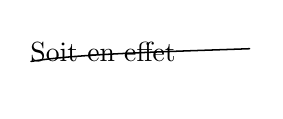
\begin{tikzpicture}[x=.20pt,y=-.20pt,baseline=(localbase),line cap=round,line join=round]
\path[use as bounding box] (0,0) rectangle (410,114);
\coordinate (localbase) at (0,61);
\begin{scope}[shift={(-285,-68)}]
\node[anchor=base west,inner sep=0pt,outer sep=0pt] at (290,129) {\rlap{Soit en effet}\phantom{\deleted{Soit en effet}}};
\draw[line width=.55pt] (291,129) .. controls (374,115) and (548,111) .. (686,106);
\end{scope}
\end{tikzpicture}
% END A025-G00
Si on a $U_s\subset
% BEGIN A025-S01
% full-scan origin: (830,122); x=.20pt, y=-.20pt; local baseline: (0,57); fixed drawing rectangle: (0,0)--(91,73).
% complete candidates: \deleted{E}\Sigma_i^- ; \deleted{I}\Sigma_i^- ; \deleted{E}\Sigma_{\prime}^- ; \deleted{I}\Sigma_{\prime}^-
% local role/state qualification: Predecessor E/I unresolved; upper run head/retrace versus independent run unresolved; index i/prime unresolved. Primary candidate uses deleted E, live Sigma_i^- and head/retrace. Independent upper-run candidate has undetermined hand.
\unsure{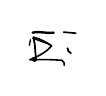
\begin{tikzpicture}[x=.20pt,y=-.20pt,baseline=(localbase),line cap=round,line join=round]
\path[use as bounding box] (0,0) rectangle (91,73);
\coordinate (localbase) at (0,57);
\node[overlay,anchor=base west,inner sep=0pt,outer sep=0pt] at (0,57) {\phantom{$\deleted{\unsure{E|I}}\Sigma_{\unsure{i|\prime}}^-$}};
\begin{scope}[shift={(-830,-122)}]
\draw[line width=.85pt] (839,131) .. controls (853,128) and (864,133) .. (877,131);
\draw[line width=.58pt] (840,139) .. controls (852,142) and (866,149) .. (873,155) .. controls (865,165) and (851,173) .. (834,180) .. controls (859,179) and (879,180) .. (892,181) .. controls (897,183) and (896,188) .. (896,190);
\draw[line width=.48pt] (835,144) .. controls (833,148) and (833,150) .. (833,154);
\draw[line width=.64pt] (841,143) .. controls (844,153) and (843,164) .. (845,176) .. controls (849,184) and (837,184) .. (839,177);
\draw[line width=.48pt] (839,141) -- (872,153);
\draw[line width=.60pt] (895,130) -- (917,132);
\draw[line width=.66pt] (902,159) .. controls (902,163) and (904,166) .. (908,168);
\end{scope}
\end{tikzpicture}}
% END A025-S01
$, $\overline{U_s}
% BEGIN A025-G01
% full-scan origin: (1099,153); x=.20pt, y=-.20pt; local baseline: (0,27); fixed drawing rectangle: (0,0)--(47,36).
% complete candidates: \deleted{=}\cap

\begin{tikzpicture}[x=.20pt,y=-.20pt,baseline=(localbase),line cap=round,line join=round]
\path[use as bounding box] (0,0) rectangle (47,36);
\coordinate (localbase) at (0,27);
\node[overlay,anchor=base west,inner sep=0pt,outer sep=0pt] at (0,27) {\phantom{$\deleted{=}\cap$}};
\begin{scope}[shift={(-1099,-153)}]
\draw[line width=.55pt] (1105,168) -- (1137,168);
\draw[line width=.50pt] (1104,175) -- (1130,176);
\draw[line width=.85pt] (1108,175) .. controls (1120,157) and (1127,153) .. (1135,164) .. controls (1140,172) and (1139,177) .. (1139,181);
\end{scope}
\end{tikzpicture}
% END A025-G01
% BEGIN A025-G02
% full-scan origin: (1159,132); x=.20pt, y=-.20pt; local baseline: (0,43); fixed drawing rectangle: (0,0)--(66,59).
% complete candidates: E_j ; E_i
% local role/state qualification: Index j primary, i retained; point retained once as the common dotted-index component. No independent-point candidate is selected.
\unsure{\begin{tikzpicture}[x=.20pt,y=-.20pt,baseline=(localbase),line cap=round,line join=round]
\path[use as bounding box] (0,0) rectangle (66,59);
\coordinate (localbase) at (0,43);
\node[overlay,anchor=base west,inner sep=0pt,outer sep=0pt] at (0,43) {\phantom{$E_{\unsure{j|i}}$}};
\begin{scope}[shift={(-1159,-132)}]
\draw[line width=.50pt] (1167,141) -- (1167,169) .. controls (1168,173) and (1175,172) .. (1195,172);
\draw[line width=.43pt] (1173,141) .. controls (1180,137) and (1193,137) .. (1199,143);
\draw[line width=.47pt] (1169,161) -- (1188,161);
\fill (1218,157) .. controls (1221,156) and (1221,160) .. (1219,162) -- (1217,161) -- cycle;
\draw[line width=.52pt] (1211,174) .. controls (1214,180) and (1214,183) .. (1209,185);
\end{scope}
\end{tikzpicture}}
% END A025-G02
\ne\varnothing$,
% BEGIN A025-G03
% full-scan origin: (1405,138); x=.20pt, y=-.20pt; local baseline: (0,39); fixed drawing rectangle: (0,0)--(136,60).
% complete candidates: \deleted{et si}
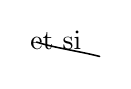
\begin{tikzpicture}[x=.20pt,y=-.20pt,baseline=(localbase),line cap=round,line join=round]
\path[use as bounding box] (0,0) rectangle (136,60);
\coordinate (localbase) at (0,39);
\begin{scope}[shift={(-1405,-138)}]
\node[anchor=base west,inner sep=0pt,outer sep=0pt] at (1410,177) {\rlap{et si}\phantom{\deleted{et si}}};
\draw[line width=.56pt] (1421,164) .. controls (1451,174) and (1501,181) .. (1535,190);
\end{scope}
\end{tikzpicture}
% END A025-G03
alors
% BEGIN A025-G04
% full-scan origin: (295,283); x=.20pt, y=-.20pt; local baseline: (0,15); fixed drawing rectangle: (0,0)--(143,22).
% complete candidates: Reduced complete phrase on a ; Three unassigned traces
% local role/state qualification: Lexical reading on a retained with low confidence; role/attachment and hand of unassigned-trace candidate undetermined.
\unsure{\begin{tikzpicture}[x=.20pt,y=-.20pt,baseline=(localbase),line cap=round,line join=round]
\path[use as bounding box] (0,0) rectangle (143,22);
\coordinate (localbase) at (0,15);
\node[overlay,anchor=base west,inner sep=0pt,outer sep=0pt] at (0,15) {\phantom{$\text{on a}$}};
\begin{scope}[shift={(-295,-283)}]
\fill (301,297) -- (303,293) -- (306,294) -- (304,297) -- cycle;
\draw[line width=.24pt] (325,296) .. controls (334,293) and (339,293) .. (343,292);
\draw[line width=.49pt] (343,292) -- (352,292) -- (357,296);
\draw[line width=.52pt] (422,295) .. controls (423,293) and (429,293) .. (432,295);
\end{scope}
\end{tikzpicture}}
% END A025-G04

\[
\begin{aligned}
U_s=X\setminus\mathop{
% BEGIN A025-G05
% full-scan origin: (847,268); x=.20pt, y=-.20pt; local baseline: (0,68); fixed drawing rectangle: (0,0)--(84,79).
% complete candidates: \rlap{\raisebox{.65ex}{$\scriptstyle-$}}\bigcup ; \deleted{\bigcap}\bigcup
% local role/state qualification: Cross presence firm; complete cross-on-union versus earlier-intersection/live-union state remains unresolved. No disjointness operation inferred.
\unsure{
\begin{tikzpicture}[x=.20pt,y=-.20pt,baseline=(localbase),line cap=round,line join=round]
\path[use as bounding box] (0,0) rectangle (84,79);
\coordinate (localbase) at (0,68);
\node[overlay,anchor=base west,inner sep=0pt,outer sep=0pt] at (0,68) {\phantom{$\unsure{\rlap{\raisebox{.65ex}{$\scriptstyle-$}}\bigcup|\deleted{\bigcap}\bigcup}$}};
\begin{scope}[shift={(-847,-268)}]
\draw[line width=.65pt] (865,275) .. controls (873,293) and (865,326) .. (880,337) .. controls (899,348) and (923,325) .. (919,285);
\draw[line width=.43pt] (853,287) .. controls (863,279) and (870,280) .. (876,291) .. controls (879,309) and (873,327) .. (883,336) .. controls (896,345) and (922,321) .. (917,282);
\draw[line width=.53pt] (857,291) .. controls (875,291) and (893,293) .. (903,290);
\draw[line width=.44pt] (912,290) -- (914,316);
\end{scope}
\end{tikzpicture}}
% END A025-G05
}\limits_{\alpha\in K}
% BEGIN A025-S02
% full-scan origin: (966,251); x=.20pt, y=-.20pt; local baseline: (0,81); fixed drawing rectangle: (0,0)--(98,98).
% complete candidates: \widehat{\Sigma}_\alpha^+ with the two locally qualified upper-index traces
% local role/state qualification: Head/body pale junction observed joined. The two small upper-index traces retain attachment, role, hand and surface-origin uncertainty separately.
\begin{tikzpicture}[x=.20pt,y=-.20pt,baseline=(localbase),line cap=round,line join=round]
\path[use as bounding box] (0,0) rectangle (98,98);
\coordinate (localbase) at (0,81);
\node[overlay,anchor=base west,inner sep=0pt,outer sep=0pt] at (0,81) {\phantom{$\widehat{\Sigma}_\alpha^+$}};
\begin{scope}[shift={(-966,-251)}]
\draw[line width=.43pt] (995,270) -- (1012,260) .. controls (1018,265) and (1022,273) .. (1033,273);
\draw[line width=.54pt] (973,291) -- (1021,287);
\draw[line width=.43pt] (975,291) .. controls (988,296) and (1002,302) .. (1007,309) .. controls (1012,316) and (984,325) .. (970,330) .. controls (997,329) and (1019,327) .. (1028,332);
\draw[line width=.52pt] (1047,284) -- (1051,304);
\draw[line width=.50pt] (1039,294) -- (1060,294);
\draw[line width=.45pt] (1047,337) .. controls (1043,326) and (1030,321) .. (1030,333) .. controls (1030,349) and (1043,342) .. (1048,330) .. controls (1051,324) and (1052,319) .. (1053,314);
\draw[line width=.51pt] (1042,331) .. controls (1046,337) and (1050,341) .. (1057,339);
% BEGIN A025-M01
% nested full-scan origin (1041,306), local baseline (0,0), base-west zero-separation anchor; owns two upper-index traces only.
\node[anchor=base west,inner sep=0pt,outer sep=0pt] at (1041,306) {\unsure{\begin{tikzpicture}[x=.20pt,y=-.20pt,baseline=(markbase)]
\path[use as bounding box] (0,0) rectangle (10,15);\coordinate (markbase) at (0,0);
\draw[gray,line width=.21pt] (1,2) -- (3,3);
\fill (3,9) -- (6,8) -- (8,11) -- (5,14) -- cycle;
\end{tikzpicture}}};
% END A025-M01
\end{scope}
\end{tikzpicture}
% END A025-S02
&\qquad\text{
% BEGIN A025-G06
% full-scan origin: (1220,295); x=.20pt, y=-.20pt; local baseline: (0,25); fixed drawing rectangle: (0,0)--(56,33).
% complete candidates: Reduced complete word où ; Three unassigned traces
% local role/state qualification: où primary; lexical attachment and alternative trace hand remain unresolved.
\unsure{\begin{tikzpicture}[x=.20pt,y=-.20pt,baseline=(localbase),line cap=round,line join=round]
\path[use as bounding box] (0,0) rectangle (56,33);
\coordinate (localbase) at (0,25);
\node[overlay,anchor=base west,inner sep=0pt,outer sep=0pt] at (0,25) {\phantom{$\text{où}$}};
\begin{scope}[shift={(-1220,-295)}]
\fill (1226,320) -- (1230,316) -- (1233,316) -- (1232,320) -- cycle;
\draw[line width=.29pt] (1241,320) -- (1256,318);
\draw[line width=.48pt] (1256,318) -- (1270,319);
\draw[line width=.43pt] (1261,302) -- (1264,309);
\end{scope}
\end{tikzpicture}}
% END A025-G06
}\quad i\in K\subset I\\
&\forall\alpha\in K\qquad
% BEGIN A025-S03
% full-scan origin: (1244,359); x=.20pt, y=-.20pt; local baseline: (0,41); fixed drawing rectangle: (0,0)--(96,54).
% local role/state qualification: Joined upper arm and body; this local head carries no independent detached-run doubt.
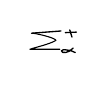
\begin{tikzpicture}[x=.20pt,y=-.20pt,baseline=(localbase),line cap=round,line join=round]
\path[use as bounding box] (0,0) rectangle (96,54);
\coordinate (localbase) at (0,41);
\node[overlay,anchor=base west,inner sep=0pt,outer sep=0pt] at (0,41) {\phantom{$\Sigma_\alpha^+$}};
\begin{scope}[shift={(-1244,-359)}]
\draw[line width=.48pt] (1251,369) -- (1304,365);
\draw[line width=.39pt] (1254,369) .. controls (1271,372) and (1294,378) .. (1295,382) .. controls (1283,389) and (1260,394) .. (1248,398) -- (1302,398);
\draw[line width=.47pt] (1320,363) -- (1324,376);
\draw[line width=.47pt] (1312,368) -- (1332,367);
\draw[line width=.48pt] (1326,396) .. controls (1319,405) and (1305,406) .. (1305,401) .. controls (1308,396) and (1317,401) .. (1321,400) -- (1330,404);
\end{scope}
\end{tikzpicture}
% END A025-S03
\in\pi_0(X\setminus E_\alpha)\ 
% BEGIN A025-G07
% full-scan origin: (1597,345); x=.20pt, y=-.20pt; local baseline: (0,37); fixed drawing rectangle: (0,0)--(71,52).
% complete candidates: \deleted{\text{les}} ; \deleted{K} ; \deleted{\text{tel}}
% local role/state qualification: les primary, K/tel retained; deletion state firm. Final rightward run reaches physical edge; no independent terminal comma observed.
\unsure{
\begin{tikzpicture}[x=.20pt,y=-.20pt,baseline=(localbase),line cap=round,line join=round]
\path[use as bounding box] (0,0) rectangle (71,52);
\coordinate (localbase) at (0,37);
\node[overlay,anchor=base west,inner sep=0pt,outer sep=0pt] at (0,37) {\phantom{$\deleted{\unsure{\text{les}|K|\text{tel}}}$}};
\begin{scope}[shift={(-1597,-345)}]
\draw[line width=.43pt] (1605,350) -- (1608,387) -- (1630,365) -- (1635,354);
\draw[line width=.43pt] (1602,369) -- (1635,353);
\draw[line width=.42pt] (1609,369) .. controls (1622,373) and (1624,375) .. (1632,374) .. controls (1642,373) and (1644,369) .. (1640,367);
\draw[line width=.39pt] (1654,367) -- (1646,381) -- (1646,386);
\draw[line width=.55pt] (1623,379) -- (1665,379);
\end{scope}
\end{tikzpicture}}
% END A025-G07
\\
&
% BEGIN A025-G08
% full-scan origin: (1103,438); x=.20pt, y=-.20pt; local baseline: (0,57); fixed drawing rectangle: (0,0)--(56,74).
% complete candidates: \deleted{U\Sigma} ; \deleted{\bigcup\Sigma} ; \deleted{U} ; U\Sigma
% local role/state qualification: Deleted U Sigma primary; alternative glyphs preserve original C row and newly retained live compound state. No chronology supplied.
\unsure{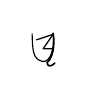
\begin{tikzpicture}[x=.20pt,y=-.20pt,baseline=(localbase),line cap=round,line join=round]
\path[use as bounding box] (0,0) rectangle (56,74);
\coordinate (localbase) at (0,57);
\node[overlay,anchor=base west,inner sep=0pt,outer sep=0pt] at (0,57) {\phantom{$\unsure{\deleted{U\Sigma}|\deleted{\bigcup\Sigma}|\deleted{U}|U\Sigma}$}};
\begin{scope}[shift={(-1103,-438)}]
\draw[line width=.42pt] (1111,449) .. controls (1112,479) and (1112,495) .. (1130,499) .. controls (1144,501) and (1152,476) .. (1149,448);
\draw[line width=.44pt] (1119,460) -- (1149,450) -- (1131,476) -- (1148,476);
\draw[line width=.59pt] (1149,448) .. controls (1153,473) and (1147,494) .. (1138,501) .. controls (1139,510) and (1146,508) .. (1152,502);
\end{scope}
\end{tikzpicture}}
% END A025-G08
\ \text{les }
% BEGIN A025-S04
% full-scan origin: (1288,437); x=.20pt, y=-.20pt; local baseline: (0,38); fixed drawing rectangle: (0,0)--(70,48).
% complete candidates: \Sigma_\alpha^+ with head/retrace ; \Sigma_\alpha^+ with independent upper run
% local role/state qualification: Detached head/body; head role locally unresolved. Recurring primary printed without second unsure. Independent-run candidate upper-hand undetermined.
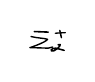
\begin{tikzpicture}[x=.20pt,y=-.20pt,baseline=(localbase),line cap=round,line join=round]
\path[use as bounding box] (0,0) rectangle (70,48);
\coordinate (localbase) at (0,38);
\node[overlay,anchor=base west,inner sep=0pt,outer sep=0pt] at (0,38) {\phantom{$\Sigma_\alpha^+$}};
\begin{scope}[shift={(-1288,-437)}]
\draw[line width=.58pt] (1300,444) -- (1325,445);
\draw[line width=.50pt] (1294,453) .. controls (1306,456) and (1319,456) .. (1324,458) .. controls (1322,462) and (1302,470) .. (1292,473) -- (1325,474) -- (1333,472);
\draw[line width=.54pt] (1346,442) -- (1349,455);
\draw[line width=.47pt] (1338,447) -- (1356,446);
\draw[line width=.56pt] (1343,468) .. controls (1352,464) and (1344,475) .. (1335,479) .. controls (1326,481) and (1331,473) .. (1339,474) -- (1354,478);
\end{scope}
\end{tikzpicture}
% END A025-S04
\ \text{mut\textsuperscript{t}. disjoints}
\end{aligned}
\]
Il faut voir que $
% BEGIN A025-G09
% full-scan origin: (874,478); x=.20pt, y=-.20pt; local baseline: (0,139); fixed drawing rectangle: (0,0)--(194,162).
% complete candidates: \deleted{K}\inserted{K\setminus\{i\}} with long run acting as guide ; \deleted{K}\inserted{K\setminus\{i\}} with long run acting as strike
% local role/state qualification: Words/state firm; long-run role remains unresolved locally, with source-positioned curved geometry.
\begin{tikzpicture}[x=.20pt,y=-.20pt,baseline=(localbase),line cap=round,line join=round]
\path[use as bounding box] (0,0) rectangle (194,162);
\coordinate (localbase) at (0,139);
\begin{scope}[shift={(-874,-478)}]
\node[anchor=base west,inner sep=0pt,outer sep=0pt] at (880,543) {$\inserted{K\setminus\{i\}}$};
\node[overlay,anchor=base west,inner sep=0pt,outer sep=0pt] at (952,615) {\phantom{$\deleted{K}$}};
\draw[line width=.45pt] (959,552) -- (973,621);
\draw[line width=.45pt] (963,590) -- (1000,564);
\draw[line width=.57pt] (969,597) -- (1000,613);
\draw[line width=.50pt] (979,548) .. controls (991,552) and (1003,540) .. (988,555) -- (962,573) .. controls (979,571) and (996,559) .. (1002,563) .. controls (1018,570) and (977,590) .. (986,600) .. controls (1011,593) and (992,619) .. (978,635);
% BEGIN A025-M02
% long guide/strike: full-scan origin (920,526), local baseline (0,0), base-west zero separation.
\node[anchor=base west,inner sep=0pt,outer sep=0pt] at (920,526) {\unsure{\begin{tikzpicture}[x=.20pt,y=-.20pt,baseline=(guidebase)]
\path[use as bounding box] (0,0) rectangle (145,101);\coordinate (guidebase) at (0,0);
\draw[line width=.28pt] (5,97) .. controls (-2,78) and (19,48) .. (42,42) .. controls (74,32) and (111,20) .. (141,6) .. controls (144,4) and (140,2) .. (136,3);
\end{tikzpicture}}};
% END A025-M02
\end{scope}
\end{tikzpicture}
% END A025-G09
$ et les $
% BEGIN A025-S05
% full-scan origin: (1236,552); x=.20pt, y=-.20pt; local baseline: (0,48); fixed drawing rectangle: (0,0)--(82,61).
% complete candidates: \Sigma_\alpha^+ with head/retrace ; \Sigma_\alpha^+ with independent upper run
% local role/state qualification: Separate upper run; its head/retrace role remains unresolved at this independent occurrence. No extra index point.
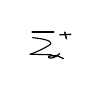
\begin{tikzpicture}[x=.20pt,y=-.20pt,baseline=(localbase),line cap=round,line join=round]
\path[use as bounding box] (0,0) rectangle (82,61);
\coordinate (localbase) at (0,48);
\node[overlay,anchor=base west,inner sep=0pt,outer sep=0pt] at (0,48) {\phantom{$\Sigma_\alpha^+$}};
\begin{scope}[shift={(-1236,-552)}]
\draw[line width=.48pt] (1244,560) -- (1283,560);
\draw[line width=.40pt] (1245,570) .. controls (1263,572) and (1279,575) .. (1278,581) .. controls (1275,585) and (1251,597) .. (1240,600) -- (1279,601);
\draw[line width=.50pt] (1303,560) -- (1306,572);
\draw[line width=.46pt] (1294,565) -- (1314,564);
\draw[line width=.44pt] (1294,599) .. controls (1285,607) and (1276,608) .. (1274,606) .. controls (1270,602) and (1286,602) .. (1290,603) -- (1301,608);
\end{scope}
\end{tikzpicture}
% END A025-S05
$ $(\alpha\in K\setminus\{i\})$ sont determinés en termes de $i$ et de $
% BEGIN A025-S06
% full-scan origin: (291,819); x=.20pt, y=-.20pt; local baseline: (0,62); fixed drawing rectangle: (0,0)--(110,76).
% complete candidates: \Sigma_i^+ with head/retrace ; \Sigma_{\prime}^+ with head/retrace ; \Sigma_i^+ with independent upper run ; \Sigma_{\prime}^+ with independent upper run
% local role/state qualification: Rising detached head; index i/prime locally retained. Recurring primaries printed after S01; independent-run candidate hand undetermined.
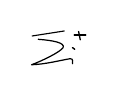
\begin{tikzpicture}[x=.20pt,y=-.20pt,baseline=(localbase),line cap=round,line join=round]
\path[use as bounding box] (0,0) rectangle (110,76);
\coordinate (localbase) at (0,62);
\node[overlay,anchor=base west,inner sep=0pt,outer sep=0pt] at (0,62) {\phantom{$\Sigma_i^+$}};
\begin{scope}[shift={(-291,-819)}]
\draw[line width=.41pt] (299,834) -- (357,825);
\draw[line width=.44pt] (310,840) .. controls (336,842) and (359,846) .. (355,855) .. controls (350,863) and (317,879) .. (298,886) .. controls (324,885) and (350,878) .. (368,875) .. controls (374,875) and (372,882) .. (372,884);
\draw[line width=.48pt] (383,826) -- (386,841);
\draw[line width=.47pt] (375,832) -- (396,832);
\draw[line width=.51pt] (372,855) -- (376,858);
\end{scope}
\end{tikzpicture}
% END A025-S06
$ i.e. $
% BEGIN A025-S07
% full-scan origin: (548,806); x=.20pt, y=-.20pt; local baseline: (0,59); fixed drawing rectangle: (0,0)--(101,69).
% complete candidates: \Sigma_i^- with head/retrace ; \Sigma_{\prime}^- with head/retrace ; \Sigma_i^- with independent upper run ; \Sigma_{\prime}^- with independent upper run
% local role/state qualification: Detached nearly horizontal head; local i/prime alternative remains recorded; recurring primary printed.
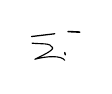
\begin{tikzpicture}[x=.20pt,y=-.20pt,baseline=(localbase),line cap=round,line join=round]
\path[use as bounding box] (0,0) rectangle (101,69);
\coordinate (localbase) at (0,59);
\node[overlay,anchor=base west,inner sep=0pt,outer sep=0pt] at (0,59) {\phantom{$\Sigma_i^-$}};
\begin{scope}[shift={(-548,-806)}]
\draw[line width=.46pt] (555,822) -- (597,817);
\draw[line width=.41pt] (556,834) .. controls (574,836) and (589,833) .. (593,842) .. controls (595,847) and (575,856) .. (561,863) .. controls (583,857) and (609,856) .. (615,865);
\draw[line width=.58pt] (621,813) -- (642,814);
\draw[line width=.52pt] (615,851) -- (616,855);
\end{scope}
\end{tikzpicture}
% END A025-S07
$. Je dis que
\[
K\setminus\{i\}=\bigl\{\alpha\in I\mid E_\alpha\subset
% BEGIN A025-S08
% full-scan origin: (1169,900); x=.20pt, y=-.20pt; local baseline: (0,55); fixed drawing rectangle: (0,0)--(103,65).
% local role/state qualification: Faint joined head/body junction; alpha and minus firm. No correction to index.
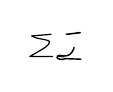
\begin{tikzpicture}[x=.20pt,y=-.20pt,baseline=(localbase),line cap=round,line join=round]
\path[use as bounding box] (0,0) rectangle (103,65);
\coordinate (localbase) at (0,55);
\node[overlay,anchor=base west,inner sep=0pt,outer sep=0pt] at (0,55) {\phantom{$\Sigma_\alpha^-$}};
\begin{scope}[shift={(-1169,-900)}]
\draw[line width=.45pt] (1176,915) -- (1211,912);
\draw[line width=.43pt] (1178,915) .. controls (1183,921) and (1204,920) .. (1208,925) .. controls (1212,932) and (1184,945) .. (1173,952) -- (1214,952);
\draw[line width=.57pt] (1239,912) -- (1264,909);
\draw[line width=.51pt] (1253,936) .. controls (1249,948) and (1243,952) .. (1233,951) .. controls (1215,946) and (1220,962) .. (1238,956) -- (1265,957);
\draw[line width=.35pt] (1224,952) -- (1235,953);
\end{scope}
\end{tikzpicture}
% END A025-S08
\]
% Lower-right detached mark group, full-scan location retained in its source declaration.
\figure{\hfill
% BEGIN A025-M03
% full-scan origin: (1591,1713); x=.20pt, y=-.20pt; local baseline: (0,15); fixed drawing rectangle: (0,0)--(16,18).
% complete candidates: Two detached graphical marks with unestablished role, attachment, hand and surface origin
% local role/state qualification: Shape preserved; no character, writer or mathematical role supplied.
\unsure{\begin{tikzpicture}[x=.20pt,y=-.20pt,baseline=(localbase),line cap=round,line join=round]
\path[use as bounding box] (0,0) rectangle (16,18);
\coordinate (localbase) at (0,15);
\begin{scope}[shift={(-1591,-1713)}]
\fill (1600,1717) .. controls (1604,1714) and (1604,1719) .. (1600,1720) -- cycle;
\fill (1595,1724) .. controls (1598,1722) and (1599,1726) .. (1596,1728) -- cycle;
\end{scope}
\end{tikzpicture}}
% END A025-M03
}
% archive sheet number: 24
